\documentclass[12pt,letterpaper]{article}
\usepackage[utf8]{inputenc}
\usepackage[T1]{fontenc}
\usepackage[spanish]{babel}
\usepackage{geometry}
\usepackage{graphicx}
\usepackage{algorithm}
\usepackage{algpseudocode}


\geometry{top=2.5cm, bottom=2.5cm, left=2.5cm, right=2.5cm}


\usepackage{fancyhdr}
\pagestyle{fancy}
\fancyhf{} 


\lhead{Luis Enrique Escamilla Rufina}
\rhead{UNAM - Facultad de Ciencias}
\cfoot{\thepage}

\renewcommand{\headrulewidth}{0.6pt} 


\title{Chat con servidor y cliente.}
\author{Luis Enrique Escamilla Rufina}

\begin{document}

\maketitle
\thispagestyle{fancy} 

\section{Resumen}
El primer proyecto de Modelado y Programación, que consiste hacer un chat con servidor y cliente (todo desde cero), mismo que debe tener un protocolo en JSON tanto servidor como cliente y que se puedan conectar entre si, sin importar en que lenguaje sean implementados, además de todo lo que implica ello, como que el servidor pueda manejar multiples clientes que mandan y reciben texto ya sea público o privado, con la creación de salas, mismas a las que solo se puede acceder si se recibe una invitación.

\section{Introducción}
Para empezar, el problema que se va a resolver es, como ya se habia mencionado anteriormente crear un chat, que básicamente es establecer una comunicación bidireccional con ayuda del manejo de sockets para el uso de red, hilos de ejecución para los multiples clientes, es decir, con uso de la programación concurrente para lograr procesar y enviar texto a multiples clientes o salas. También es importante tener en cuenta posibles riesgos como que dos hilos de ejecución quieran modificar una estructura de datos (lista o diccionario) al mismo tiempo, no borrar correctamente a un cliente cuando se desconecte y provocar que se desperdicie memoria del servidor.

Alguna limitación algo importante es que el uso del cliente se hace mediante la línea de comandos de la terminal, lo cual siento que puede ser hasta cierto punto confuso, ya que si contara con una interfaz gráfica sería mucho más fácil y con una vista despejada para usar el cliente del chat junto al hecho de no usar prefijos para cada acción. Otro punto interesante sería agregar una estructura que permitiera guardar los mensajes para que al cerrar el cliente y después abrirlo, los mensajes sigan ahí (algo así como hacen las aplicaciones de mensajería de hoy en día).

Un punto que se podría considerar como ``ayuda'' es desde mi caso, tener un conocimiento básico sobre como funciona un servidor pequeño gracias a las clases de Introducción a Ciencias de la Computación, y gracias a esto no tener una gran dificultad en como (al menos) empezar con una prueba pequeña del servidor para que desde ahí continuar con lo importante de este proyecto.


\newpage
\section{Análisis y Diseño}
Para comenzar con la primera parte que es hacer el análisis del problema, fue con leer el protocolo y en general tratar de entender aunque sea un poco que es lo que se pide que haga cada instrucción, además tomé como referencia para basarme mayormente el servidor realizado en primer semestre, siendo la lógica que éste realiza cuando llega un cliente y como procesa las peticiones que haga el mismo.

Con esto, y que el servidor solo se dedique a mantener la lista de clientes, haga o borre las salas (que no lleven el mismo nombre), saber que clientes pertenecen a ella para poder invitar a más gente, evitar como se habia dicho que dos hilos modifiquen la lista de clientes y provocar inconsistencias y que los mensajes puedan llegar a sus destinos correctamente, sean privados o públicos, también de ser capaz de mantener a multiples clientes con su identificación y el estado de cada quien (una parte de informacion de ellos), además de nombres de usuarios que sean válidos (no más de 8 caracteres), que no se repitan entre varios, que puedan saber quienes más están conectados en una sala o en el chat general por defecto, y saber cuando alguien se desconecta para que sea borrado de la lista de clientes y notificarlo a los demás

Teniendo en cuenta esto, para el protocolo y las distintas opciones que hay para interactuar con él, decidí en separarlo como distintos tipos de ``modos'', a manera de que quedara como, lo que el servidor recibe, lo que se quiere hacer y el resultado de lo que se hace, además de los distintos tipos de estados que puede tener un cliente/usuario, en si, que procese los diferentes tipos u operaciones del protocolo. De igual forma es necesario tener algo que pueda saber el nombre de un cliente, su estado en el chat, saber las salas en las que pueda estar dentro, que sea capaz de poder armar y desarmar el mensaje en JSON y lo más importante que controle la comunicación tanto en el servidor como en el cliente y que se pueda lograr que cada usuario este aislado.

Para el lado del cliente, elegí usar una estructura similar a la que empecé a plantear en el servidor, pero haciendo una distinción importante y es que mientras el servidor solo recibe conexiones, procesa las solicitudes y enviar el texto a los diferentes usuarios, esta parte del proyecto es la que haga la conexión con el servidor y evite que el usuario tenga que escribir el JSON tal cual en la terminal, basicamente se reduzca a solo escribir algo con un prefijo y asi poder internamente convertirlo a la solicitud que se desee y al formato del protocolo para que sea enviado al servidor, además de que esto mismo pueda distinguir lo que otros clientes hagan, como cambiar su estado, mandarle un mensaje privado o uno público, una invitación para una sala o que se desconecten, así como también mostrar errores que pueda cometer el usuario, en general, presentarle los resultados de una forma clara.

Como sucedió con el servidor, aquí se pueden distinguir partes necesarias para realizar este lado, como enviar y recibir los mensajes del servidor para que sean procesados o simplemente mostrados dependiendo de su operación, procesar un prefijo y armar la parte del protocolo correspondiente para enviarlo, y asi poder tener un cliente que sin importar como sea implementado, mientras maneje de forma correcta el protocolo pueda hacerlo con otro servidor.



\newpage
\subsection*{Diseño del servidor}
Con la parte del análisis obtenida para el servidor, resultó en una separación de trabajo que considero buena para realizar el diseño del mismo, debido a que el proceso principal del servidor solo debe de recibir conexiones, revisar y procesar los mensajes del protocolo, junto con la administración de las salas y los mensajes que se envíen tanto en estas como en privado (dos clientes) o público (sala general). Investigando para esto, descubrí que hay un patrón de diseño llamadado ``Mediador'', en el que todos los que se conectan al medidador y él procesa la lógica y decide a donde dirigir el siguiente paso de la información, el cual, considero que en parte es bastante util para el servidor.

Como el servidor debe manejar multiples clientes, lo mejor es que al recibir un cliente se le da un hilo de ejecución con el propósito de que no se vea afectados a los demás clientes en su manejo de solicitudes, además de crearle una conexión asociada a cada uno para que desde ahí se pueda manejar su estado, su lista de salas, y poder tener su identificación mediante el nombre que decidan ponerse. A partir de aquí cuando se recibe un mensaje mediante su conexión, se ``desarma'' y se decide que se quiere hacer.

En este caso, para poder representar los distintos mensajes que usa el protocolo pensé en una clase que tenga los distintos tipos de mensajes y estados solo como texto, para que así se pueda tener un poco más de control a la hora de armar la respuesta del servidor a los clientes y dividida en tres partes, una que tenga las operaciones que se le pueden pedir al servidor, como mandar texto, identificarse, crear salas, o abandonar el chat general por mencionar algunos, otra parte contiene los resultados que dan las operaciones anteriores ya sea exitoso, que un usuario con el mismo nombre ya existe, o que si no poder unirse a una sala que no existe, etc, además otra que contiene los tipos del protocolo como IDENTIFY, TEXT, etc, por último tambien una que representa los diferentes estados que hay en el chat como ACTIVE que se asigna por defecto al crear una conexión.

Junto a lo anterior tambien faltaría una clase que se encarge de armar en parte el mensaje del protocolo, en esta vendrían las diferentes nombres de las operaciones, como el nombre de la sala, el nombre de un usuario. Evidentemente estas no siempre son obligatorias/están por lo que son opcionales para que así se pueda seriar en JSON lo unico que sí está en el mensaje, esto es más que nada como una forma de representar internamente al protocolo

\begin{figure}[htbp]
  \centering
  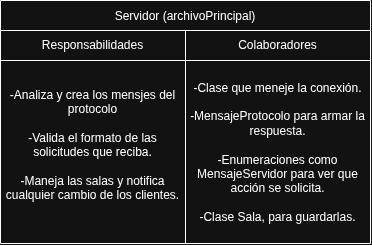
\includegraphics[width=0.5\textwidth]{CrcServirdordrawio.png}
  \caption{Responsabilidades del servidor.}
  \label{fig:fig1}
\end{figure}

\newpage
Con la figura anterior podemos describir brevemente el algoritmo que sigue el servidor, con la responsabilidad de validar el formato y que analíza las solicitudes, siguiendo el patrón de diseño mediador, cuando la clase encargada de la conexión le envía una operación ya desarmada (o deserializada del JSON) el servidor revisa el mensaje para decidir que hacer después, esto mediante un método que procese el mensaje, ahí mismo el primer paso es tener una verificación en el servidor, ya que, de lo contrario se hace una desconexión para evitar dar paso a lo que el cliente quiera hacer como mandar mensaje público, cambiar su estado, crear una sala, invitar a alguien a su sala, etc.

La responsabilidad de crear mensajes, es mediante el uso de la clase MensajeProtocolo (mencionada anteriormente como la que define el nombre de las operaciones), si es una acción que sí se pudo completar se hace un mensaje con la respuesta, apoyandose de la clase que contiene las operaciones, lo que se quiere hacer y el resultado como lo pide el protocolo, se le manda a la clase encargada de la conexión, esta la serializa en JSON y la manda o muestra al cliente (aplica lo mismo cuando es un error)

Con el tema de las salas y en como se notifica o reparte el mensaje de cambio de un usuario, se tiene una clase sala que dentro de ella tiene un diccionario que guarda sus usuarios propios, la cual solo empieza a existir si se pide una sala. La notificación se hace de una manera sencilla con el diccionario que tiene el servidor sobre todos los clientes o conexiones que recibe con ayuda de nuevo del gestor de conexiones.

\newpage
\subsection*{Diseño del cliente}
Para el diseño del cliente apoyandome de lo anterior dado por el análisis, en parte ya tenía algo para esta parte porque como pensé en reusar por lo menos las clases que arman el formato del JSON con el que tiene las operaciones y lo que se hace ahora desde el cliente y sabiendo que es desde mi punto de vista es como lo inverso del servidor (de alguna forma me hizo sentido verlo así) en donde se procesa la solicitud para recibirla o enviarla al servidor, y mostrar al usuario.

Decidí tener como en el servidor el manejo de la conexión que ahora es el que conecta a él y recibe o manda los mensajes pero más corto, el cual solo se encarga de desarmar y armar el protocolo. También una clase encargada de procesar o controlar estos mensajes, unicamente realiza la interpretación del prefijo para armar un mensaje de salida y lo manda a la conexión que a su vez lo manda al servidor, otra cosa importante que también hace es que después de recibir un mensaje ya deserializado del protocolo verifica en que caso cae y le dice a la vista que debe mostrarle al cliente, clase la cual solo se dedica a esto; mostrar las instrucciones iniciales, además de los mensajes, cambios de estado, invitaciones, etc.

\begin{figure}[htbp]
  \centering
  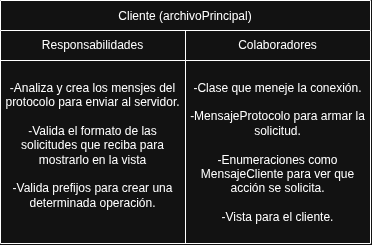
\includegraphics[width=0.5\textwidth]{CrcClientedrawio.png}
  \caption{Responsabilidades del cliente.}
  \label{fig:fig2}
\end{figure}

Para describir el algoritmo del cliente en contraste con el del servidor, es bastante corto y sencillo. Para recibir mensajes, lo atrapa la conexión lo deserializa del protocolo y un método que procese el mensaje de acuerdo al tipo de opereación le dice a la vista que debe mostrar en la terminal al cliente. Al enviar mensajes, cuando el cliente escribe un prefijo y todo lo que ello implique, por ejemplo para identificarse como |Prefijo| y |Nombre|, un método que verifique si lo que se recibe desde la terminal empiece con un prefijo en especifico, después dependiendo de cual sea va a caer en una operación y empezará a armar el mensaje del protocolo con ayuda de la clase MensajeProtocolo, el cual lo que haga se pasa a la clase que gestiona la conexión, misma que se encarga de seriarlo en JSON y de mandarlo al servidor para que este haga el algoritmo ya descrito antes.

Básicamente tienen una forma de trabajar cliente-servidor muy parecida en cuestión del manejo del protocolo pero a la vez totalmente separados para que puedan funcionar (espero) en cualquier otro servidor o cliente.

\newpage
\section{Implementación}
La implementación del proyecto decidí hacerlo completamente en C\# ya que su sintáxis es algo familiar con lo que había trabajado en los primeros dos semestres y con ayuda de Meson como sistema de construcción.

Un primer detalle que noté al hacer pruebas con el lenguaje es que al compilarlo deja como un ejecutable un .exe, lo cual pues no me gustó y busqué si habia formas de poder cambiar el resultado de compilar y encontré que C\# tiene algo llamado ``NativeAOT'' o en sus siglas en inglés ``Ahead-of-Time'' que como dice su nombre permite compilar el código directamente a código de maquina nativo, en lugar de su compilación habiatual. Un detalle es que una de sus limitaciones es que elimina algo llamado ``Reflexión'', es decir, no se puede generar código en tiempo de ejecución y fue una cosa que en un inicio no le di mucha importancia.

Para poder empezar a implementar primero el servidor, el lenguaje tiene en sus clases herramientas que son útiles para este tipo de funcionanmiento en la red como TcpListener y TcpClient para usarlo en la conexión, además de que para manejar las listas de los clientes, o mejor dicho diccionarios hay una biblioteca llamada Collections.Concurrent y en especial el ConcurrentDictionary, lo que lo hace valioso porque en él no hay necesidad de usar explícitamente en la clase del Servidor o de la Conexión cosas como ``lock'' o ``''synchronized'' de Java por ejemplo, si no que lo hace la estructura dentro de ella, por lo que ahorra bastante tiempo en tratar de como hacer funcionar cosas como bloques de ``lock'' o relacionado.

En sí, el servidor escucha en el puerto que reciba, crea un hilo de ejecución que lleva a ese cliente a un método llamado nuevoCliente, el cual, le hace una instacia de la clase Conexión, y el primer paso como cliente o usuario es identificarse para que el diccionario de clientes empiece a ser llenado. Para leer de los datos y escribir en los sockets, hay cosas como StreamReader y StreamWriter que ayudan mucho con esto, además de forzar su escritura por la red con AutoFlush para que no ocurra  en un momento de que no aparecía nada en la terminal por no tener esta opción activa, 

Para poder sacar el contenido del protocolo, hice uso de la biblioteca System.Text.Json además de su variante Json.Serialize, para hacer la clase MensajeProt (recortada en parte del nombre original MensajeProtocolo), con la que se le incluyen configuraciones como [JsonPropertyName] para definir el nombre de las operaciones y [JsonIgnore] para que campo que no se llene sea ignorado y no se incluya en el mensaje final para que siga siendo válido. La clase mas sencilla es MensajeServidor, donde solo son 4 enumeraciones donde se incluye cosas como IDENTIFY, NEW-USER, USERS, conocida como MensajeServidor, otra donde estan las acciones como TEXT, JOIN-ROOM, LEAVE-ROOM, que es conocida ahora como MensajeHacer, una tercera que solo tiene las respuestas del Servidor como SUCESS, INVALID, NO-SUCH-ROOM, etc que fue llamada MensajeResultado, y por último una en donde solo se tienen los 3 posibles estados de un cliente como ACTIVE, AWAY o BUSY, siendo esta MensajeEstado.

Con todo esto el funcionamiento del servidor se resume en un método principal llamado procesaMensaje que es un switch que revisa desde el enumerador Tipo de MensajeProt al lo que recibe, pero antes de cualquier cosa, verifica que el que manda el mensaje sea alguien ya dentro de la lista de clientes y que el mensaje esté bien definido, de lo contrario se le hace una desconexión, y si pada esto evalua en algun método en concreto como identificaCliente por ejemplo.

\newpage
También tiene una forma de protección, en la que si ocurren caso de IOException con bloque try-catch o finally siempre se hace una desconexión segura que borre a los clientes y le notifica a los demás creando un MensajeProt con Tipo, Hacer, Extra, etc(que aqui forma los mensajes o avisos, incluso invitaciones) que al final manda a la Conexión, la cual al ser creada le asigna a los clientes el estado ACTIVE, y cuando un cliente se registra se le asigna ese nombre a su conexión, además de tener su propio ConcurrentDictionary para las salas en las que pueda estar y ser invitado, cosa que se vuelve como una característica de esta clase y se queda fuera del conocimiento por defecto del servidor, hasta que acceda a eso.

Como se decía anteriormente, esta clase se encarga primero al recibir, de deshacer el JSON con su metodo JsonSerialize.Deserialize para que sea revisado por el switch del servidor, además del metodo contrario .Serialize. Aquí fue donde encontré un detalle importante, al usar la AOT por más  que mi protocolo según yo estuviera bien, siempre obtenia el resultado ``Mensaje inválido'' que le había puesto al servidor, lo cual es el detalle que menciono antes sobre que la reflexión no se puede usar en este modo de compilación y por lo tanto no se puede saber las propiedades y tipos de las clases dinámicamente en tiempo de ejcución de la biblioteca .Text.Json, ya que AOT elimina código que considera no se va a usar para reducir tamaño, al crear algo llamado JsonSerializerContext se le indica al compilador que genere el código de serialización durante el tiempo de compilación y se usa como argumento del método que serializa como del que deserializa.

Finalmente si el proceso de convertir a MensajeProt falla o se manda un JSON malo se desconecta al cliente mediante un método que cierra los flujos de lectura y escritura y de cerrar de igual forma el socket, para evitar desperdiciar memoria en general.

Para la implementación del cliente resulta más sencillo, tomando las clases MensajeProt y la enumeración MensajeServidor ahora llamada MensajeCliente para seguir de forma parecida la lógica del servidor pero en el cliente.

El primer paso es que para evitar que el cliente se bloquee esperando a que se reciba algo, (similar a esperar a recibir una conexión) el cliente delega esto a un thread para escuchar el teclado y otro que solo escucha del servidor para presentarlo en pantalla.

Como dije, para no tener que escribir todo el protocolo, metí una serie de prefijos como |=ALL <texto> para poder mandar mensaje públicos esto mediante una instancia de MensajeProt, el cual solo se llena con lo que sea necesario para cumplir esa parte del protocolo y en su clase Conexión que solo recibe y manda los mensaje se serializa el mensaje en JSON para que sea mandado al servidor.

Al recibir mensajes es algo similar, ya que recibe la cadena seriada y en la conexión la deserializa y lo pasa por un switch llamado procesaProtocolo (procesaProt más corto) y de ahi le dice a la vista como mostrarlo solo mediante Console.WriteLine(). Como pasa en el servidor se tiene un try - catch por si se cierra el servidor o similar se le notifica al cliente y desconecta de forma segura, junto con terminar la ejecución del mismo.

\newpage
\section{Conclusión}
Creo que hacer este proyecto desde cero aplicando el modelo de la cascada lo hace un poco más complejo, ya que hay que tener en cuenta casos en donde algo puede salir mal y tratar de tener lo mejor posible cada etapa para no tener que regresarse y corregir problemas, además de que sin querer desde el principio ``amarré'' el análisis al lenguaje C\# para según yo no tener que hacer demás cosas creo que resulta la mejor idea. Además de que use como base el servidor de Introducción a Ciencias de la Computación aparte de tener una idea, siento que me hizo comprender mejor ese tema de primer semestre de la red y los hilos de ejecución, ya que implementar desde cero vi algunas cosas que en ese momento no fue así y pues la verdad se me hizo muy interesante implementar el protocolo con JSON ya que nunca lo había visto como tal pero si escuchado en internet, asi que por lo menos ya tengo conocimiento de lo que es.


\subsection{Bibliografia}
Microsoft. (s.f.). Reflection vs. source generation in System.Text.Json. Microsoft Learn. de https://learn.microsoft.com/en-us/dotnet/standard/serialization/system-text-json/reflection-vs-source-generation

Microsoft. (s.f.). Implementación de AOT nativo. Microsoft Learn.  de https://learn.microsoft.com/es-es/dotnet/core/deploying/native-aot/

Gurovich, EV (2012). Introducción a las Ciencias de la Computación con JAVA. Universidad Nacional Autónoma de México. Facultad de Ciencias
\end{document}
